\documentclass[10pt,twocolumn,letterpaper]{article}

\usepackage{cvpr}
\usepackage{times}
\usepackage{epsfig}
\usepackage{graphicx}
\usepackage{amsmath}
\usepackage{amssymb}
\usepackage{epstopdf} %% EPS to PDF

%\usepackage{tikz}
%\usepackage{pgfplots}

%\DeclareGraphicsExtensions{.png,.tex}
%\graphicspath{{figs/}}

%\pgfplotsset{compat=}

% Include other packages here, before hyperref.

% If you comment hyperref and then uncomment it, you should delete
% egpaper.aux before re-running latex.  (Or just hit 'q' on the first latex
% run, let it finish, and you should be clear).
\usepackage[breaklinks=true,bookmarks=false]{hyperref}

\cvprfinalcopy % *** Uncomment this line for the final submission

\def\cvprPaperID{****} % *** Enter the CVPR Paper ID here
\def\httilde{\mbox{\tt\raisebox{-.5ex}{\symbol{126}}}}

% Pages are numbered in submission mode, and unnumbered in camera-ready
%\ifcvprfinal\pagestyle{empty}\fi
\setcounter{page}{1}
\begin{document}

%%%%%%%%% TITLE
\title{Tiny ImageNet Challenge: Project Milestone}

\author{Jose Krause Perin\\
Stanford University\\
{\tt\small jkperin@stanford.edu}
% For a paper whose authors are all at the same institution,
% omit the following lines up until the closing ``}''.
% Additional authors and addresses can be added with ``\and'',
% just like the second author.
% To save space, use either the email address or home page, not both
}

\maketitle
%\thispagestyle{empty}

%%%%%%%%% ABSTRACT
\begin{abstract}
This milestone report presents preliminary results of the Tiny ImageNet Challenge using a proposed convolutional neural network architecture based on VGG-16. The highest accuracy on the training set was $47.3\%$, while the highest accuracy in the validation set was $33.46\%$. This large gap between training and validation accuracies indicates that the performance of the network can be improved by using overfitting prevention techniques such as regularization and dropout. I plan to address this issue in the remainder of the quarter. 
\end{abstract}

%%%%%%%%% BODY TEXT
\section{Introduction}
% Introduction: this section introduces your problem, and the overall plan for approaching your problem

The Tiny ImageNet challenge has similar format to the ImageNet Large Scale Visual Recognition Challenge (ILSVRC) \cite{ILSVRC15}, which is a well-known image classification and localization benchmark for large scale datasets. As the name suggests, however, the Tiny ImageNet Challenge has a much smaller data set. There are a total of 200 classes. Each class has 500 $64\times 64$ training images, yielding a total of 100,000 images. The validation and testing data sets have a total of 10,000 $64\times 64$ images. 

The ultimate goal is to design a convolutional network architecture that achieves the highest classification accuracy possible on the test data set.

This milestone report describes the best convolutional neural network that I have designed so far and presents results in terms of loss and classification accuracy. The remainder of this report is organized as follows. Section 2 presents the problem statement. Section 3 describes the technical approach and the convolutional neural network architecture. Section 4 presents preliminary results and discussion.

\section{Problem statement}
% Describe your problem precisely specifying the dataset to be used, expected results and evaluation
The data and evaluation metric for this problem are already well defined. The data was provided on the class website, and the ultimate goal is to design a network architecture that achieves the highest accuracy on the test data set. 

In this report, I quantify the performance of the network in terms of the loss and classification accuracy vs training epoch on the training and validation data sets. These curves can provide insights on how well learning is progressing and indicate issues such as whether the learning rate is appropriate or whether there is significant over fitting. 

The output uses a Softmax layer with categorical cross-entropy loss. Hence, as there are 200 different classes or categories, the initial loss of a randomly initialized network should be about $\ln(200) \approx 5.298$.  

\section{Technical Approach}
% Describe the methods you intend to apply to solve the given problem

Before we can start training the neural network, the training, validation, and testing data sets must be loaded from JPEG files and preprocessed. This pre-processing has the goal of making the input vectors zero mean and confined between $[-1, 1]$, as the back-propagation algorithm works better under such conditions. The mean image was calculated by averaging all images from the training set. 

The convolutional network model was built and trained using Keras \cite{keras} with Tensorflow backend. Keras is a high-level deep learning library that allows us to easily build and test network architectures without having to worry about ``house keeping'' from Tensorflow. 

The proposed convolutional neural network architecture is based on the VGG-16, and it is summarized in Table~\ref{tab:network} network architecture. The number of convolutional and max pooling layers is different from VGG-16, since the VGG-16 is designed for $224 \times 224$ images (after cropping), while the images for the Tiny ImageNet Challenge were $64\times 64$. Moreover, differently from VGG-16, I added dropout layers after convolutional layers to mitigate over fitting. However, as shown by the results in Section 4, the network still experiences considerable over fitting.

All convolutional layers had stride of one and padding of one in order to preserve the image shape from their input. Moreover, all convolutional layers had a $3\times 3$. All Conv2 and fully connected layers had ReLU activation.

The MaxPool layers had $2\times 2$ window with no padding and stride 2, which resulted in down-sampling the input by a factor of 2. 

After the convolutional layers, there were three fully connected layers intercalated by $50\%$ dropout layers. 

The weights were initialized according to the uniform Glorot initializer \cite{glorot2010}, whereby the weights are uniformly distributed in a range determined by the fan-in and fan-out of the particular layer. The biases are initialized with zeros. 

\begin{table}[t]
	\caption{Network architecture. All Conv2 and fully connected layers had ReLU activation.}
	\label{tab:network}
	\centering
	\begin{tabular}{c|c}
		\hline
		Layer & Input shape \\
		\hline
		Conv2-128 $3\times 3$ & $64\times64\times 3$ \\
		Conv2-128 $3\times 3$ & $64\times64\times 128$ \\
		MaxPool $2 \times 2$ & $64\times64\times 128$\\
		\hline
		Conv2-256 $3\times 3$ & $32\times32\times 128$ \\
		Conv2-256 $3\times 3$ & $32\times32\times 256$ \\
		Dropout $50\%$ & $32\times32\times 256$ \\
		MaxPool $2 \times 2$ & $32\times32\times 256$\\
		\hline
		Conv2-512 $3\times 3$ & $16\times16\times 256$ \\
		Conv2-512 $3\times 3$ & $16\times16\times 512$ \\
		Dropout $50\%$ & $16\times16\times 512$ \\
		MaxPool $2 \times 2$ & $16\times16\times 512$\\
		\hline
		Fully connected 2048 & $32768\times 1$ \\
		Dropout $50\%$ & $2048 \times 1$ \\
		Fully connected 2048 & $2048\times 1$ \\
		Dropout $50\%$ & $2048 \times 1$ \\
		Fully connected 200 & $2048\times 1$ \\
		\hline
		Softmax & $200 \times 1$  \\
		\hline
	\end{tabular}
\end{table}

\section{Preliminary Results}
The performance of the network architectuere presented in the previous section is show in Figs~\ref{fig:loss} and \ref{fig:accu}. 

The model was trained during 20 epochs, with a stochastic gradient descent with moment 0f 0.9 and learning rate of 0.03. 

The highest accuracy on the training set was $47.3\%$, while the highest accuracy in the validation set was $33.46\%$. This large gap between training and validation accuracies indicates that the performance of the network can be improved by using over fitting prevention techniques such as regularization and dropout.

In addition to experimenting with other network architectures, for the remainder of the quarter, I plan to incorporate L2 regularization to mintage overfitting problem. I also plan to cross-validate the dropout probability to reduce overfitting. 

\begin{figure}[t!]
	\centering
	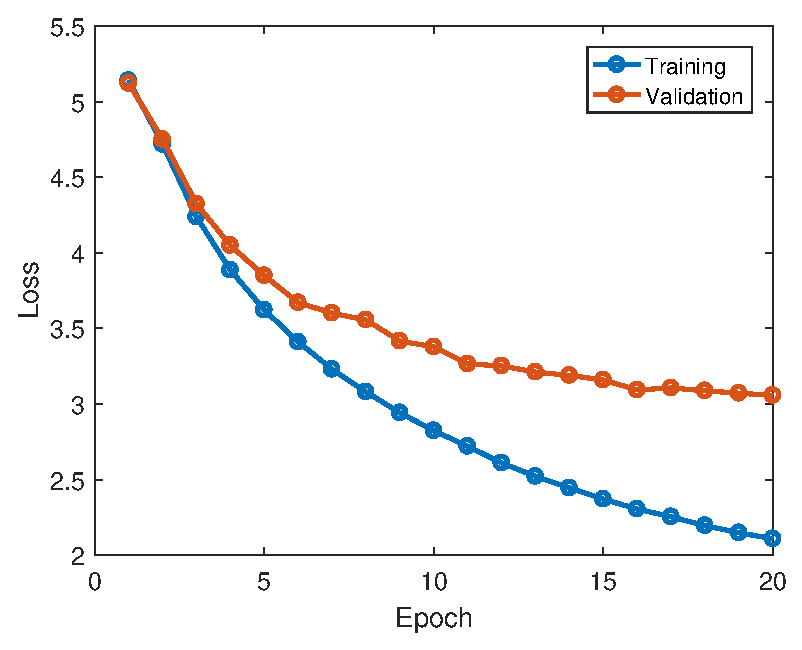
\includegraphics[width=\linewidth]{figs/milestone_loss.eps}
	\caption{Loss history on training and validation sets.}
	\label{fig:loss}
\end{figure}

\begin{figure}[t!]
	\centering
	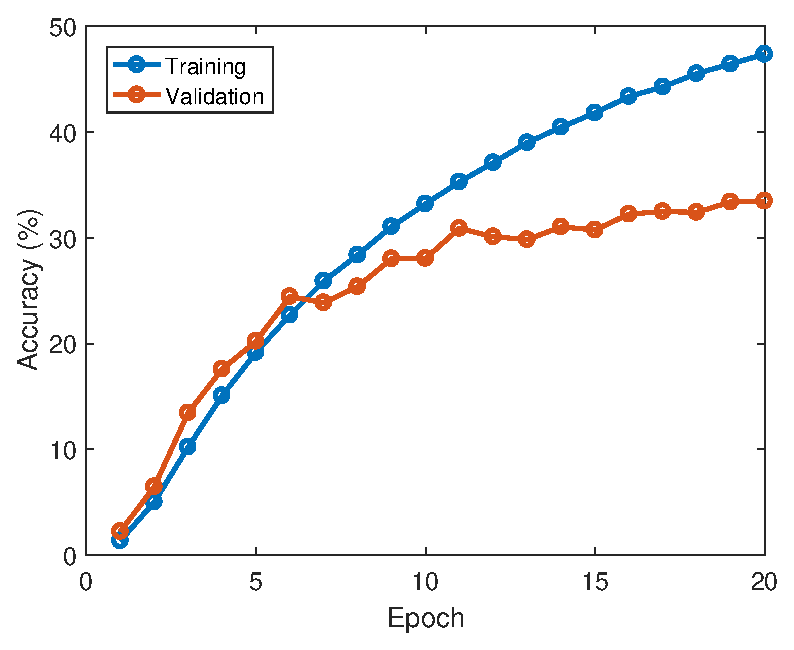
\includegraphics[width=\linewidth]{figs/milestone_accuracy.eps}
	\caption{Classification accuracy on training and validation sets.}
	\label{fig:accu}
\end{figure}



{\small
\bibliographystyle{ieee}
\bibliography{bib}
}

\end{document}
